\section{Программная реализация}

Реализованы два алгоритма обновления спинов. Односпиновый и кластерный апдейт. Оба алгоритма работают на произвольном графе, используя таблицу соседей. Алгоритмы реализованы как отдельные библиотеки для Python, и написаны с использованием технологии Cython для ускорения работы. Кластерный апдейт является более эффективным по времени работы и количеству шагов, которые необходимо выполнить для хорошей сходимости модели.

Запуск алгоритмов по симуляции модели проводились на суперкомпьютерном кластере ВШЭ Charisma. 

\subsection{Проверка алгоритмов}

Чтобы убедиться, что алгоритмы работают правильно, мы проверили, что оба алгоритма дают одинаковые результаты на одних и тех же конформациях, так же сравнил их с точными решениями для одномерной модели Изинга.

Результаты замеров кластерным и односпиновым апдейтом совпадают в пределах погрешности.

\begin{figure}[H]
	\centering
	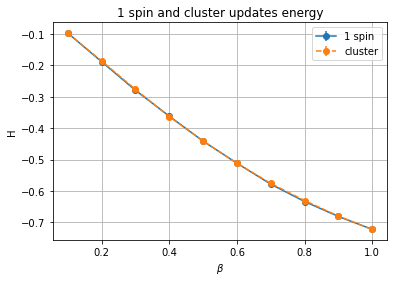
\includegraphics[width = 0.45\textwidth]{../images/1spin_&_cluster_ene.png} 
	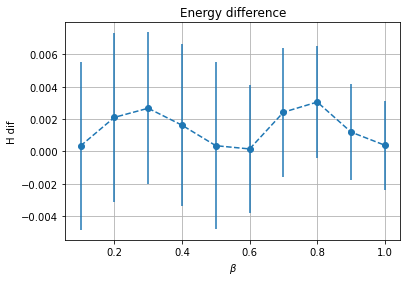
\includegraphics[width = 0.45\textwidth]{../images/1spin_&_cluster_ene_dif.png} 
	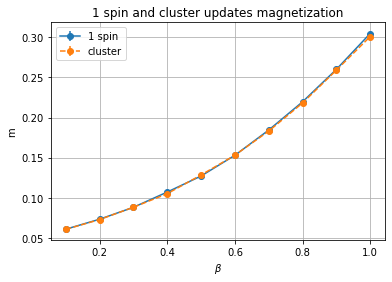
\includegraphics[width = 0.45\textwidth]{../images/1spin_&_cluster_mag.png} 
	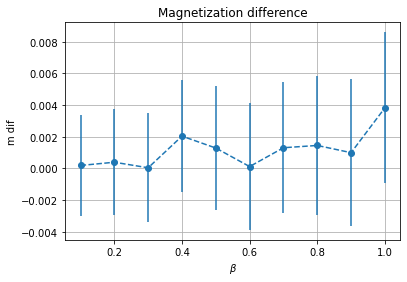
\includegraphics[width = 0.45\textwidth]{../images/1spin_&_cluster_mag_dif.png} 
	%% add magnetization
	\caption{кластерный и односпиновый апдейт}
\end{figure}

Для сравнения с точными значениями для одномерной модели Изинга, мы используем замкнутый квадратный контур. Данная конформация по свойствам полностью совпадает с одномерной моделью Изинга с открытыми граничными условиями.

\begin{figure}[H]
	\centering
	\begin{subfigure}[t]{0.45\textwidth}
		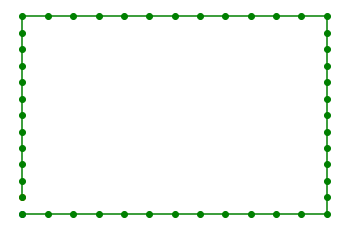
\includegraphics[width = \textwidth]{../images/1D_conf.png} 
		\caption{Конформация имитирующая одномерную модель}
	\end{subfigure}
	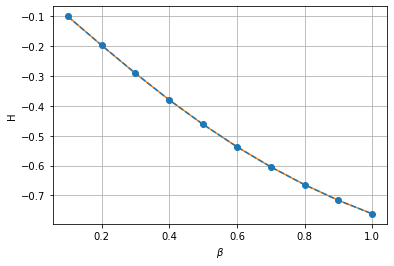
\includegraphics[width = 0.45\textwidth]{../images/1D_ene.png}
	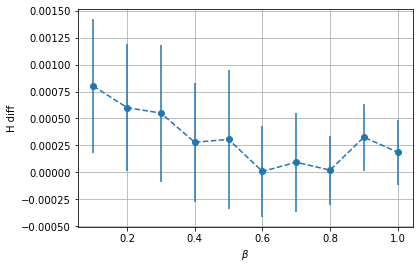
\includegraphics[width = 0.45\textwidth]{../images/1D_ene_diff.png} 
	%% add magnetization
	\caption{Сравнение с точным решением одномерной модели}
\end{figure}

Так же был написан код, точно вычисляющий энергию системы путём полного перебора всех её состояний. Сравнение на маленьких конформациях (длина до 10) даёт одинаковые результаты.



Примеры с использованием кластерного апдейта добавлены в библиотеку \texttt{mc\_lib}.